% This document should describe, in detail, how to use the device
\section{Device Operation} \label{device-operation}

\subsection{Bluetooth Commands}

\begin{flushleft}
    The ESP32 responds to 2 specific Bluetooth LE GATT commands, a Control characteristic and a Data characteristic.
\end{flushleft}

\begin{center}
    \begin{tabular}{ |l|l|l|l| }
        \hline 
        \footnotesize Characteristic & \footnotesize UUID & \footnotesize Value Handle & \footnotesize Permissions \\
        \hline 
        \scriptsize Control & \scriptsize 0000abc0-0000-1000-8000-00805f9b34fb & \scriptsize 0x002a & \scriptsize R, W \\
        \hline 
        \scriptsize Data & \scriptsize 0000abc1-0000-1000-8000-00805f9b34fb & \scriptsize 0x002d & \scriptsize R, W, N \\
        \hline
    \end{tabular}
\end{center}

\subsubsection{Station Start - Sequence diagram}

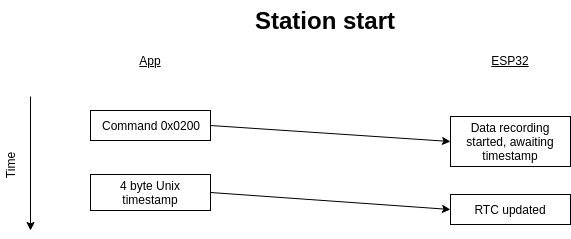
\includegraphics[scale=0.63]{buoy-rtc.png}

\subsubsection{Data Collection - Sequence diagram}

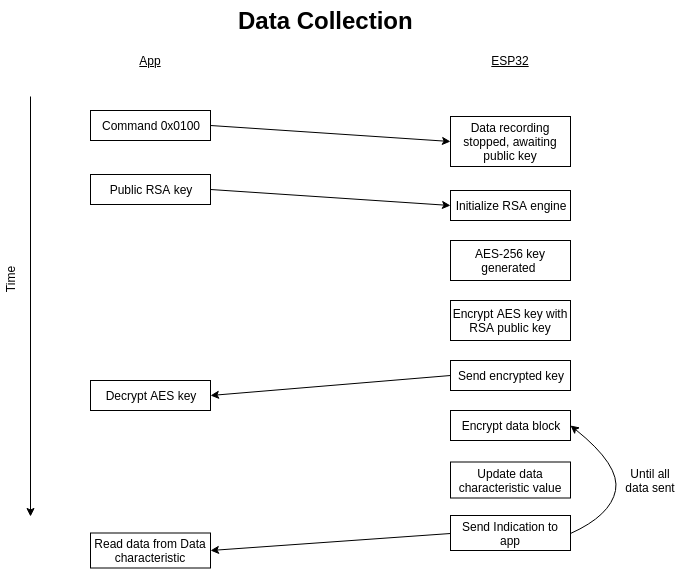
\includegraphics[scale=0.63]{buoy-data.png}

\subsection{Powering On and Connecting to the buoy}

When protoypting, connecting the Micro USB cable to the ESP32 development board to power up the device with 5 volts.
When using the production buoy, make sure 2 AA batteries are in the battery pack. Switch the power switch to ON.
Once the buoy is receiving power, it will boot up and initialize the Bluetooth Low-Energy after which the Android app may connect to the buoy through Bluetooth.